
%!TEX root=total.tex

\newcommand\comment[1]{}

\section{An Equivalent Graph Problem}

We can represent a testing scheme ${\cal S}$ for the coin-weighing problem by a graph $G_{\cal S}$ as follows: 
\begin{enumerate}
\setlength{\itemsep}{0pt}
\item It contains $\pa + \pb$ vertices, where each vertex represents a distinct coin.
\item Two vertices are joined by an edge if and only if ${\cal S}$ compares the two corresponding coins.  
\end{enumerate}
Note that we cannot gain extra information by comparing the same pair of coins twice;  WLOG, we assume that each pair of coins are compared at most once.

\begin{definition}
For a coin-weighing problem with $\pa$ real coins and $\pb$ fake coins, 
we say a testing scheme ${\cal S}$ is \emph{foolproof} if no matter how $\pa$ vertices in $G_{\cal S}$ 
are assigned as real and the remaining vertices are assigned as fake, $G_{\cal S}$ contains at least 
an \emph{unbalanced} edge whose endpoints are with different labels;  else, ${\cal S}$ is \emph{non-foolproof}.
\end{definition}

Suppose that $\pa = 3$ and $\pb = 5$.  Figure~\ref{fig:foolproof} shows two different foolproof schemes, while Figure~\ref{fig:nonfoolproof} shows a non-foolproof scheme.

\begin{figure}[!htb]
  \centering
  \begin{subfigure}[b]{0.45\textwidth}
    \centering 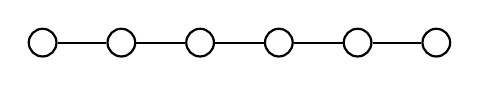
\begin{tikzpicture}[auto, thick]
\tikzstyle{vertex}=[draw,circle,text=violet,minimum width=10pt]
  \foreach \place/\name in {{(0,0)/a},
                            {(1,0)/b},
                            {(2,0)/c},
                            {(3,0)/d},
                            {(4,0)/e},
                            {(5,0)/f}}
    \node[vertex] (\name) at \place {};
  \foreach \source/\dest in {a/b,b/c,c/d,d/e,e/f}
      \path (\source) edge (\dest);
\end{tikzpicture} \vspace*{2.5ex}
    \caption{A scheme with 5 comparisons}
  \end{subfigure}
  \begin{subfigure}[b]{0.45\textwidth}
    \centering 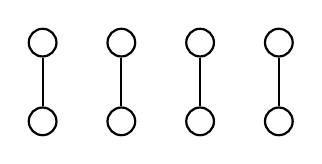
\begin{tikzpicture}[auto, thick]
\tikzstyle{vertex}=[draw,circle,text=violet,minimum width=10pt]
  \foreach \place/\name in {{(0,0)/a},
                            {(0,1)/b},
                            {(1,0)/c},
                            {(1,1)/d},
                            {(2,0)/e},
                            {(2,1)/f},
                            {(3,0)/g},
                            {(3,1)/h}}
    \node[vertex] (\name) at \place {};
  \foreach \source/\dest in {a/b,c/d,e/f,g/h}
      \path (\source) edge (\dest);
\end{tikzpicture}
    \caption{A scheme with 4 comparisons}
  \end{subfigure}
  \caption{Two foolproof schemes for $\pa = 3$ and $\pb = 5$.  Isolated vertices are omitted for brevity.} \label{fig:foolproof}
\end{figure}

\begin{figure}[!htb]
   \centering
    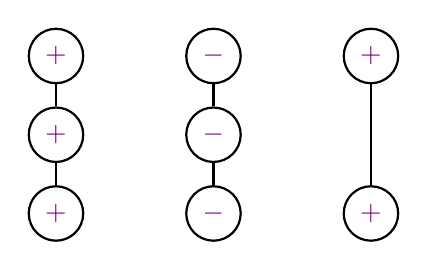
\begin{tikzpicture}[auto, thick]
\tikzstyle{vertex}=[draw,circle,text=violet,minimum width=15pt]
  \foreach \place/\name in {{(0,0)/a},
                            {(0,1)/b},
                            {(0,2)/c},
                            {(4,0)/g},
                            {(4,2)/h}}
    \node[vertex] (\name) at \place {$+$};
  \foreach \place/\name in {{(2,0)/d},
                            {(2,1)/e},
                            {(2,2)/f}}
    \node[vertex] (\name) at \place {$-$};
  \foreach \source/\dest in {a/b,b/c,d/e,e/f,g/h}
      \path (\source) edge (\dest);
\end{tikzpicture} \vspace*{2.5ex}
    \caption{A non-foolproof scheme for $\pa = 3$ and $\pb = 5$:  
                 If the leftmost $\pa$ vertices are assigned as real, there is no unbalanced edge.} \label{fig:nonfoolproof}
\end{figure}

\medskip

Let ${\cal G}(\pa,\pb)$ be a graph formed by the union of two cliques $K_\pa$ and $K_\pb$ of sizes $\pa$ and $\pb$, respectively.  We have the following theorem.

\begin{theorem} \label{thm:graph}
A testing scheme ${\cal S}$ is foolproof if and only if $G_{\cal S}$ is not isomorphic to any subgraph of ${\cal G}(\pa,\pb)$. 
\end{theorem}
\begin{proof}
Suppose that $G_{\cal S}$ is isomorphic to some subgraph of ${\cal G}(\pa,\pb) = K_\pa \cup K_\pb$. 
Then, we may select an arbitrary isomorphism, and label as real for all those $\pa$ vertices in $G_{\cal S}$ that are mapped to the vertices in $K_\pa$, while label as fake for the remaining $\pb$ vertices.  Under such a labeling, there will be no unbalanced edge, so that ${\cal S}$ is non-foolproof.

\smallskip

Conversely, if ${\cal S}$ is non-foolproof, there exists a way to label $\pa$ vertices in $G_{\cal S}$ as real and the remaining $\pb$ vertices as fake so that there is no unbalanced edge.  In other words, $G_{\cal S}$ can be partitioned into two sugraphs with $\pa$ and $\pb$ vertices, respectively;  the former one is isomorphic to a subgraph of $K_\pa$ and the latter one is isomorphic to a subgraph of $K_\pb$,  so that $G_{\cal S}$ is isomorphic to a subgraph of ${\cal G}(\pa,\pb)$.
\end{proof}

\begin{definition}
For a coin-weighing problem with $\pa$ real coins and $\pb$ fake coins, 
we say a foolproof testing scheme ${\cal S}$ is \emph{optimal} if it requires the minimal number of 
comparisons in the worst case;  the minimal number of comparisons is denoted by $\tau(\pa,\pb)$.
\end{definition}
\noindent
{\it Remark.} By  definition, $\tau(\pa,\pb) = \tau(\pb,\pa)$.

\bigskip

The target of this paper is to design optimal foolproof testing scheme so that by comparing coins according to the scheme, we are guaranteed to compare a real coin with a fake coin using the fewest comparisons in the worst case.  By Theorem~\ref{thm:graph}, it is equivalent to finding a graph $G$, with the fewest number of edges, that is not isomorphic to any subgraph of ${\cal G}(\pa,\pb)$. 

\comment{
Intuitively, if finding unbalance in a comparison, the game ends. But sometimes we can point a pair is unbalance after k comparisons(k is the answer) before the unbalance appears. The following shows $k_{min}=t_{min}-1$, which means the answer for Problem 4 is $t_{min}-1$

\begin{lemma}
$t_{min} = k_{min}+1 $
\end{lemma}

\begin{proof}
We divide the proof of the equation into two inequations

If we could point out a pair $e$ is unbalanced through the optimal graph $F$(with $k_{min}$ comparisons).
Consider a graph with these $k_{min}$ edges + $e$ which is not a subgraph of ${\cal G}(\pa,\pb)$
\[t_{min}\leq k_{min}+1\]

For a optimal graph $E$(with $t_{min}$ edges) which is not a subgraph of ${\cal G}(\pa,\pb)$. Let $E'$ = ($E$ remove an arbitrary edge $e$), then through $E'$. If $E'$ has unbalance comparison, we conclude the one is unbalanced, otherwise we could conclude $e$ is unbalanced.
Either case shows $E'$ is enough to end the game.
\[k_{min} \leq t_{min}-1\]

From the above inequations, the lemma holds.

\end{proof}


In this case, testing a pair is enough to point out a real coin and a fake one. 

Denote the coins we test as $coin_a$ $coin_b$ , the coin we didn't test as $coin_c$
If $coin_a$ and $coin_b$ is not balanced, then point out $coin_a$ and $coin_b$. Otherwise, point out $coin_a$ and $coin_c$
}


\subsection{Lower Bound}

\begin{theorem} \label{thm:graph-lowerbound}
Any graph with $n \leq \pa + \pb$ vertices and $m \leq \lfloor (\pa+\pb)/2 \rfloor-1$ edges 
is always isomorphic to some subgraph of ${\cal G}(\pa,\pb)$.
\end{theorem}

\begin{proof}
Without loss of generality, we assume that $\pa \leq \pb$.  We shall prove this theorem by induction on the sum $\pa + \pb$. 

\medskip

\noindent
{\bf (Basis Case:)} If $\pa = \pb =1$, then $\lfloor (\pa+\pb)/2 \rfloor-1 = 0$. Any graph with $n \leq 2$ vertices and $m \leq 0$ edges (i.e., no edges) is always isomorphic to some subgraph of ${\cal G}(1,1)$.

\medskip

\noindent
{\bf (Inductive Case:)} Suppose that the theorem holds for all $\pa + \pb \leq k$.  Our target is to show that the theorem also holds for the case $\pa + \pb = k + 1$ with $\pa \leq \pb$.   Consider a graph $G$ with  $n \leq k+1$ vertices and with $m \leq \lfloor (k+1)/2 \rfloor -1$ edges. 

\begin{enumerate}
  \item If $G$ is connected, then $n \leq m + 1 \leq (k+1)/2 \leq b$, which is isomorphic to some subgraph of $K_\pb$, 
           and thus isomorphic to some subgraph of ${\cal G}(\pa,\pb)$.   

  \item Otherwise, $G$ is not connected.  
           If $G$ has no edges, then $G$ is obviously isomorphic to some subgraph of ${\cal G}(\pa,\pb)$ 
           since $G$ has at most $\pa+\pb$ vertices.
           Else, let $C$ be the connected component of $G$ with the largest number $n'$ of vertices (so that $n' \geq 2$.
          Then, the number of edges in $C$ is at least $n'-1$.  To complete the proof, it is sufficient to show 
          that $G - C$ is isomorphic to some subgraph of ${\cal G}(\pa, \pb - n')$, 
         as we can map the vertices of $C$ to an arbitrary set of $n'$ vertices in the $K_\pb$ component of ${\cal G}(\pa,\pb)$.

The number of vertices in $G-C$ is $k+1-n' = \pa + (\pb-n')$, and the number of edges of $G-C$ is at most 
\begin{eqnarray*}
m - (n'-1) \leq \floor{(k+1)/2} - n' &=& \floor{(k+1)/2 - n'} \\
&=& \floor{ (k+1-n')/2 - n'/2 } \\
&\leq& \floor{ (k+1-n')/2 - 1 } \\
&=& \floor{(k+1-n')/2} - 1 = \floor{ (\pa + (\pb+n'))/2 } - 1.
\end{eqnarray*}
By induction hypothesis, $G-C$ is isomorphic to a subgraph of ${\cal G}(\pa, \pb-n')$, 
and consequently $G$ is isomorphic to some subgraph of ${\cal G}(\pa,\pb)$.
\end{enumerate}
In both cases, $G$ is isomorphic to a subgraph of ${\cal G}(\pa,\pb)$.  
This completes the proof of the induction case, so that by the principle of mathematical induction, the theorem follows.
\end{proof}

Immediately, we have the following corollaries.

\begin{corollary} \label{cor:lowerbound}
For any $\pa$ and $\pb$, $\tau(\pa,\pb) \geq \lfloor(\pa+\pb)/2 \rfloor$.
\end{corollary}
\begin{proof}
The corollary is a direct consequence of Theorems~\ref{thm:graph} and~\ref{thm:graph-lowerbound}.
\end{proof}

\begin{corollary}
When $\pa$ and $\pb$ are both odd, $\tau(\pa,\pb)= (\pa+\pb)/2$.
\end{corollary}
\begin{proof}
Consider a testing scheme ${\cal S}$ that partitions the coins into $(\pa+\pb)/2$ pairs, and then compares each pair of coins.
The corresponding graph $G_{\cal S}$ consists of $(\pa+\pb)/2$ disjoint edges (as in Figure~\ref{fig:foolproof}(b)), 
and is not isomorphic to any subgraph of ${\cal G}(\pa,\pb)$.  Thus, $G_{\cal S}$ is foolproof, and $\tau(\pa,\pb) \leq (\pa+\pb)/2$.  On the other hand, by Corollary~\ref{cor:lowerbound}, we have $\tau(\pa,\pb) \geq (\pa+\pb)/2$ for odd 
$\pa$ and odd $\pb$.  The corollary thus follows.
\end{proof}

\begin{corollary} 
Consider a testing scheme ${\cal S}$ whose corresponding graph $G_{\cal S}$ forms a path with $\max(\pa,\pb) + 1$ nodes (as in Figure~\ref{fig:foolproof}(a)).  Then, ${\cal S}$ is foolproof, and it uses at most twice the number of comparisons 
of any optimal foolproof scheme.  
\end{corollary}
\begin{proof}
The graph $G_{\cal S}$ is not isomorphic to any subgraph of  ${\cal G}(\pa,\pb)$, so that it is foolproof.  The number of comparisons by ${\cal S}$ is 
\begin{eqnarray*}
\max(\pa,\pb) &\leq& \pa + \pb - 1 \ \ \ \ \ \ \ \ \ \ =\ \ \ 2 \times ( (\pa + \pb - 1)/2 ) \\
&\leq& 2 \times \lfloor (\pa + \pb)/ 2 \rfloor \ \ \leq\ \ \  2 \times \tau(\pa,\pb),
\end{eqnarray*}
where the last inequality comes from Corollary~\ref{cor:lowerbound}.  The corollary thus follows.
\end{proof}